\section{剖分的代数}
\sourcepage{111--112}
现在研究剖分的代数后果，确定它对同调群的作用。将证明：对任意复形 $K$ 及其剖分 $K'$，存在唯一确定的链映射 $\lambda:C_p(K)\to C_p(K')$，称为\textbf{剖分算子}（subdivision operator），它诱导同调同构。此外，若 $g:K'\to K$ 为底空间恒等映射的任意单纯逼近，则 $\lambda,g_\#$ 互为链同伦逆，所以 $g_*$ 也是同构。\translatornote{原文此句写 $g_\#$ 为同构；这里应指诱导的同调映射 $g_*$。}

\entry{引理}{2.5.1}设 $K'$ 为 $K$ 的剖分，则恒等映射 $i:|K|\to|K|$ 有单纯逼近 $g:K'\to K$。若 $\tau\in K'$、$\sigma\in K$ 且 $\tau\subset\sigma$，则 $g(\tau)\subset\sigma$。

\noindent\textbf{证明：}由引理 2.3.2，单纯逼近存在。给定 $\tau\subset\sigma$，若 $w$ 为 $\tau$ 的顶点，它位于 $\sigma$ 或其某个面的内部，由引理 2.2.2，$g(w)$ 为 $\sigma$ 的顶点。\hfill$\square$

\entry{定义}{2.5.2}对 $\sigma\in K$，令 $K(\sigma)$ 为由 $\sigma$ 及其各面组成的子复形，令 $K'(\sigma)$ 为 $K'$ 中多胞体等于 $\sigma$ 的子复形。

\entry{定理}{2.5.3（代数剖分定理）}设 $K'$ 为 $K$ 的剖分。存在唯一的保持增广链映射 $\lambda:\mathcal C(K)\to\mathcal C(K')$，使每个 $\lambda(\sigma)$ 都由 $K'(\sigma)$ 承载。若 $g:K'\to K$ 为恒等映射的单纯逼近，则 $\lambda,g_\#$ 互为链同伦逆，故 $\lambda_*,g_*$ 都为同构。称 $\lambda$ 为\textbf{剖分算子}。

\noindent\textbf{证明：第一步。}先在下述额外条件下证明定理：对每个 $\sigma\in K$，诱导剖分 $K'(\sigma)$ 无环。使用几何形式的无环载体定理 1.14.10。

先定义 $K\to K$ 的载体 $\Psi(\sigma)=K(\sigma)$，以及 $K\to K'$ 的载体 $\Lambda(\sigma)=K'(\sigma)$。前者无环，因为由一个单形及其面组成；后者根据额外假设无环。面包含条件也显然成立。

为定义从 $K'$ 出发的两个载体，对于 $\tau\in K'$，令 $\sigma_\tau$ 为包含 $\tau$ 的最低维 $K$ 单形。若 $t$ 为 $\tau$ 的面，则 $\sigma_t\subset\sigma_\tau$：两者的交包含 $t$，由 $\sigma_t$ 的最小维数，它必须等于此交。令
\[
\Theta(\tau)=K(\sigma_\tau),\qquad\Phi(\tau)=K'(\sigma_\tau).
\]
两者均无环，面包含条件由上述包含关系得到。图 2.5.1 展示了 $K'=\operatorname{sd}K$ 的情形。
\begin{center}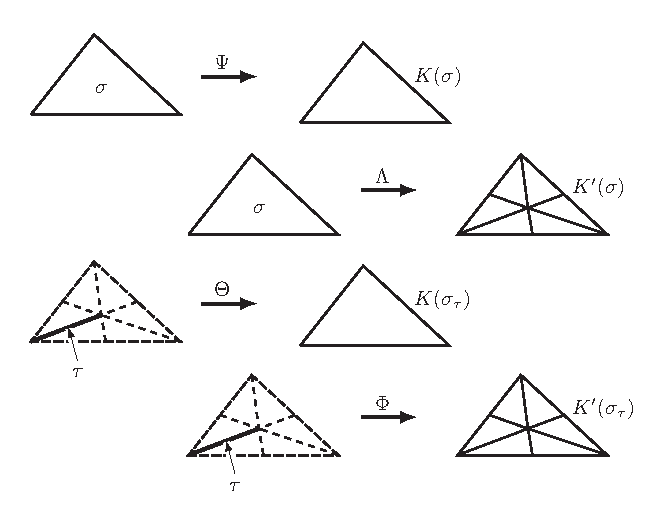
\includegraphics[width=116mm]{figures/2-5-1.pdf}\\图 2.5.1\end{center}
由无环载体定理，存在分别由 $\Lambda,\Theta$ 承载的保持增广链映射
\[
\lambda:\mathcal C(K)\to\mathcal C(K'),\qquad
\theta:\mathcal C(K')\to\mathcal C(K).
\]

\sourcepage{113--114}
$\mathcal C(K)$ 的恒等映射显然由 $\Psi$ 承载，复合 $\theta\lambda$ 也如此，因此两者链同伦。具体地，$\lambda(\sigma)$ 是 $K'(\sigma)$ 的链，其中每个单形 $\tau$ 都位于 $\sigma$ 内，故 $\sigma_\tau$ 是 $\sigma$ 或其面。因此 $\theta(\tau)$ 由 $K(\sigma_\tau)\subset K(\sigma)$ 承载，$\theta\lambda(\sigma)$ 也由 $K(\sigma)$ 承载。

同样，$\mathcal C(K')$ 的恒等映射由 $\Phi$ 承载，因为 $\tau\subset\sigma_\tau$，故 $\tau\in K'(\sigma_\tau)$。复合 $\lambda\theta$ 也由 $\Phi$ 承载：$\theta(\tau)$ 是 $\sigma_\tau$ 的各定向面的和，每个面 $s$ 的像 $\lambda(s)$ 由 $K'(s)\subset K'(\sigma_\tau)$ 承载。因此 $\lambda\theta$ 链同伦于恒等映射。

上述论证与所选择的具体 $\theta,\lambda$ 无关。$\theta$ 的一个选择是 $g_\#$，由前一引理它由 $\Theta$ 承载。所以 $g_\#,\lambda$ 互为链同伦逆。

再证唯一性。若 $\lambda'$ 为另一个由 $\Lambda$ 承载的保持增广链映射，则存在同样由 $\Lambda$ 承载的链同伦 $D$。对 $p$ 维单形 $\sigma$，$K'(\sigma)$ 维数为 $p$，而 $D\sigma$ 是由其承载的 $(p+1)$ 维链，只能为零。因此 $D=0$，由链同伦等式得 $\lambda=\lambda'$。

\textbf{第二步。}证明 $K'=\operatorname{sd}K$ 时成立。对 $\sigma\in K$，$K'(\sigma)$ 为锥 $\widehat\sigma*J$，其中 $J$ 为边界的第一次重心剖分，所以由定理 1.9.6 无环。［零维情形为单点复形。］这正是证明必须使用重心剖分之处。

\textbf{第三步。}证明 $K'=\operatorname{sd}^NK$ 时成立。由第一步，只需证明每个 $\operatorname{sd}^NK(\sigma)$ 无环。由第二步，对任意复形 $L$，
\[
\widetilde H_i(L)\cong\widetilde H_i(\operatorname{sd}L)
\cong\widetilde H_i(\operatorname{sd}^2L)\cong\cdots.
\]
所以 $L$ 无环时，其各次重心剖分也无环。

\textbf{第四步。}证明一般情形。仍只需证明任意诱导剖分 $K'(\sigma)$ 无环。令 $L=K(\sigma)$、$L'=K'(\sigma)$，已知 $L$ 无环，要证明 $L'$ 无环。取恒等映射的单纯逼近 $g:L'\to L$。由有限单纯逼近定理，选择 $N$ 使恒等映射有单纯逼近 $f:\operatorname{sd}^NL\to L'$；类似地，再选择 $M$，使其有逼近 $k:\operatorname{sd}^M(L')\to\operatorname{sd}^NL$。得到
\[
\operatorname{sd}^M(L')\xrightarrow{k}\operatorname{sd}^NL
\xrightarrow{f}L'\xrightarrow{g}L.
\]
\sourcepage{115--116}
复合 $gf$ 为恒等映射的单纯逼近，由第三步，$g_*f_*$ 为同构；同理 $f_*k_*$ 为同构。前者说明 $f_*$ 单射，后者说明它满射，因此 $f_*$ 为同构。于是 $g_*$ 也为同构，故 $L'$ 无环。\hfill$\square$

\entry{定义}{2.5.4}当 $K'=\operatorname{sd}K$ 时，将剖分算子记为 $\operatorname{sd}:C_p(K)\to C_p(\operatorname{sd}K)$，称为\textbf{重心剖分算子}。这里滥用记号，同时以 sd 表示代数与几何剖分算子。

它有归纳公式：
\[
\operatorname{sd}(v)=v,\qquad
\operatorname{sd}(\sigma)=[\widehat\sigma,\operatorname{sd}(\partial\sigma)].
\]
括号记号与第 1.9 节相同，此公式的验证留作习题。

\subsection*{在相对同调中的应用}
上述结果直接推广到相对同调。

\entry{定理}{2.5.5}设 $K_0$ 为 $K$ 的子复形，$K'$ 为 $K$ 的剖分，$K'_0$ 为其诱导的 $K_0$ 剖分。算子 $\lambda$ 诱导链映射
\[
\lambda:C_p(K,K_0)\to C_p(K',K'_0).
\]
若 $g:(K',K'_0)\to(K,K_0)$ 为恒等映射的任意单纯逼近，则 $\lambda,g_\#$ 互为链同伦逆。

\noindent\textbf{证明：}验证第一步中的各载体保持相应子复形。若 $\sigma\in K_0$，则 $\Psi(\sigma)=K(\sigma)$、$\Lambda(\sigma)=K'(\sigma)$ 分别为 $K_0,K'_0$ 的子复形。若 $\tau\in K'_0$，则它位于 $K_0$ 的某个单形中，因此包含它的最低维单形 $\sigma_\tau$ 属于 $K_0$。所以 $\Theta(\tau),\Phi(\tau)$ 也分别为 $K_0,K'_0$ 的子复形。

故 $\lambda,\theta$ 诱导相对链映射，而复合与恒等映射之间的链同伦也诱导相对链同伦。可选 $\theta=g_\#$，所以相对层次上 $g_\#,\lambda$ 互为链同伦逆。\hfill$\square$

\subsection*{习题}
\begin{enumerate}
\item 设 $K'$ 为 $K$ 的剖分，$\lambda$ 为剖分算子，$g:K'\to K$ 为恒等映射的单纯逼近。证明 $g_\#\lambda$ 等于 $C_p(K)$ 的恒等映射。
\item 图 2.5.2 中 $K,K'$ 的共同底空间为正方形区域。
\begin{enumerate}[label=(\alph*)]
\item 求剖分算子 $\lambda:C_p(K)\to C_p(K')$ 的公式。
\item 找出两个不同的恒等映射单纯逼近 $g,g':K'\to K$，说明代数剖分定理中的链等价 $\theta$ 不唯一。
\item 验证 $\lambda g_\#$ 不等于 $K'$ 链群上的恒等映射。
\end{enumerate}
\begin{center}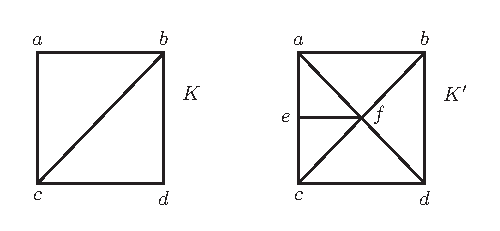
\includegraphics[width=90mm]{figures/2-5-2.pdf}\\图 2.5.2\end{center}
\item \begin{enumerate}[label=(\alph*)]
\item 证明重心剖分算子的归纳公式定义了由 $\Lambda$ 承载的保持增广链映射。
\item 对 $1$ 维、$2$ 维单形分别计算 $\operatorname{sd}\sigma$。
\end{enumerate}
\item 设 $K$ 为五边形区域［一维图形］，$K'$ 为同一五边形区域由两条对角线划分而成的复形。对它们回答习题 2(a)、(b)、(c)。\translatornote{原文写作“a pentagonal region square [the 1-dimensional figure]”，文字与维数说明互相矛盾。这里保留其意向而不擅自指定新的复形；若意在类比习题 2，应取同一填充五边形的两种剖分。}
\end{enumerate}
